\documentclass[12pt, a4paper]{article}
\usepackage{../notesheets}

%%%%%%%%%%%%%%%%%%%%%%%%%%%%%%%%%%%%%%%%%%%%%%%%%%
\author{Math 1210}
\title{Notesheet. Section 2.5 (Continuity) Part I}
\date{}

\begin{document}
\maketitle
\nameline
%%%%%%%%%%%%%%%%%%%%%%%%%%%%%%%%%%%%%%%%%%%%%%%%%%
\begin{examp}
  The function whose graph is depicted below is \textit{not} continuous at $x = a$, $b$, $c$, nor $d$.  At all other values of $x$, the function is continuous. \\\\

  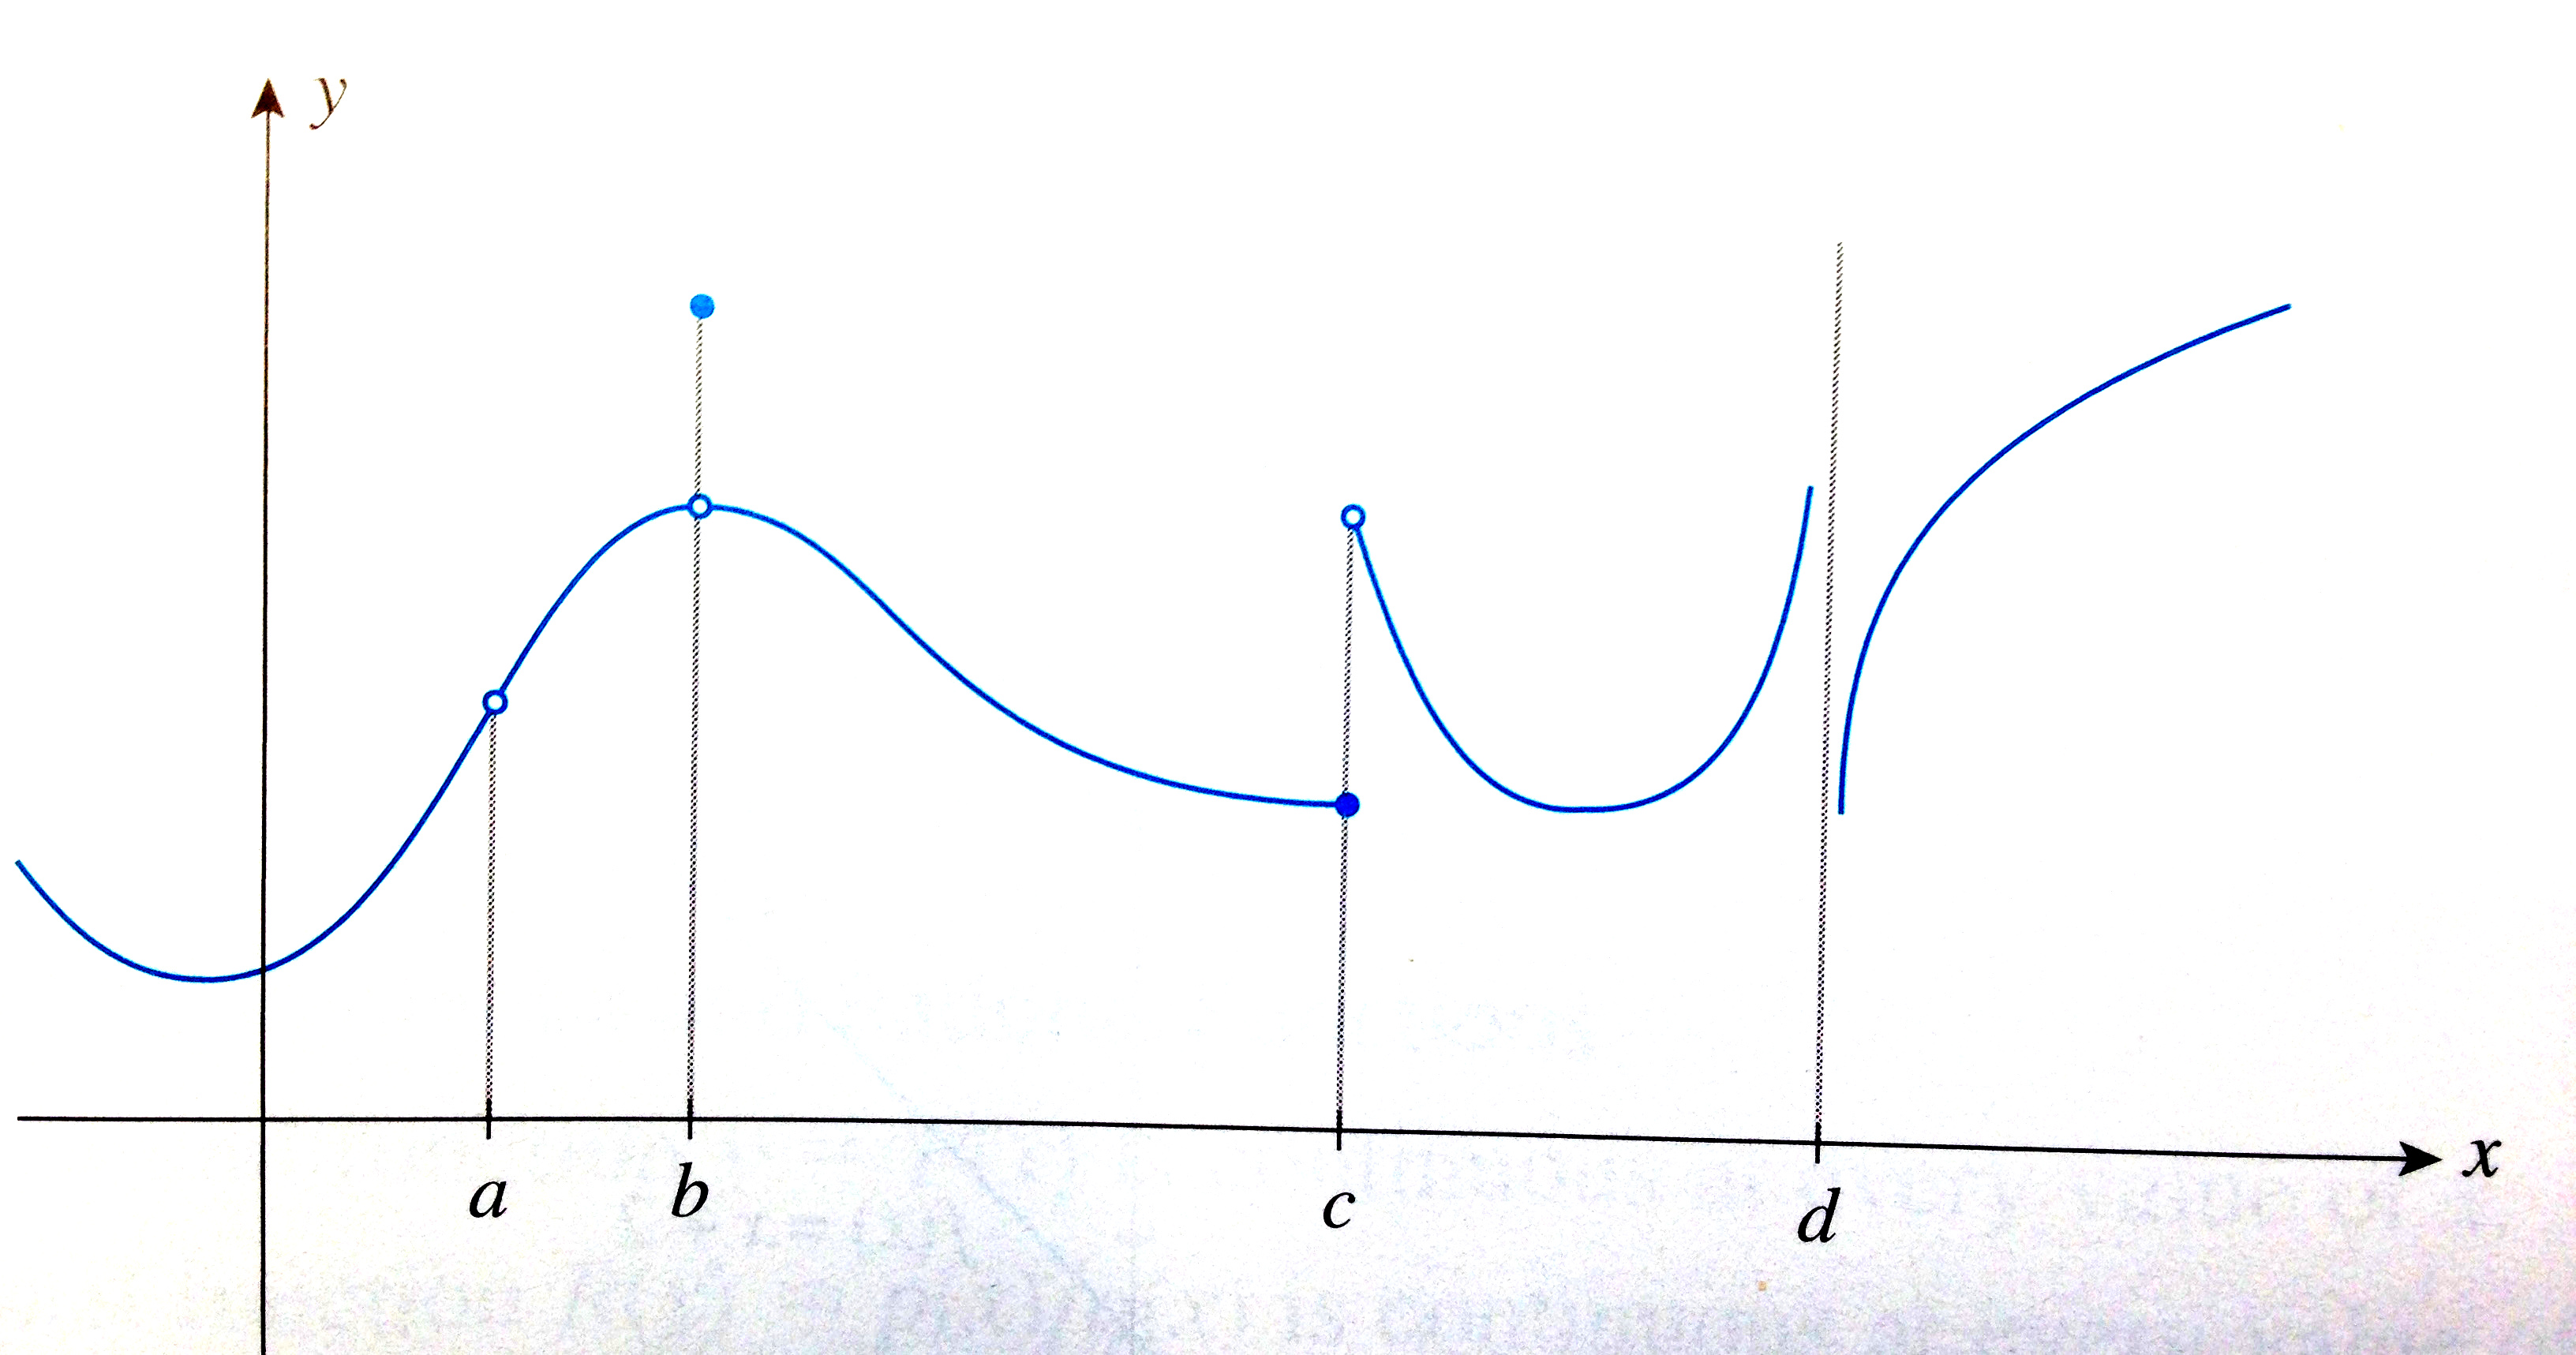
\includegraphics[scale=0.09]{images/non-continuous-examples-contrast}
\end{examp}
\begin{defi}
  A function $f$ is continuous at a number $x = a$ if the following 3 conditions are satisfied:
\end{defi}
\begin{defi}
  Given a function \(f(x)\), when is \(f(x)\) \textbf{discontinous} at
  a point? When is \(f(x)\) \textbf{continuous on an interval}?
\end{defi}
\begin{ex}
  Find the values of $x$ for which each function is continuous.  Use interval notation when appropriate.
  \begin{enumerate}
    \item $f(x) = \frac{x^2 - 49}{x + 7}$
    \item $h(x) = \begin{cases}
      1 &\text{if $x < 0$} \\
      \frac{x + 2}{2} &\text{otherwise}
    \end{cases}$
  \end{enumerate}
\end{ex}
\begin{ex}
  Is the function graphed below continuous at $-1$?  Is it continuous
  at $1$?  At $2$?  At $4$? At \(5\)?

  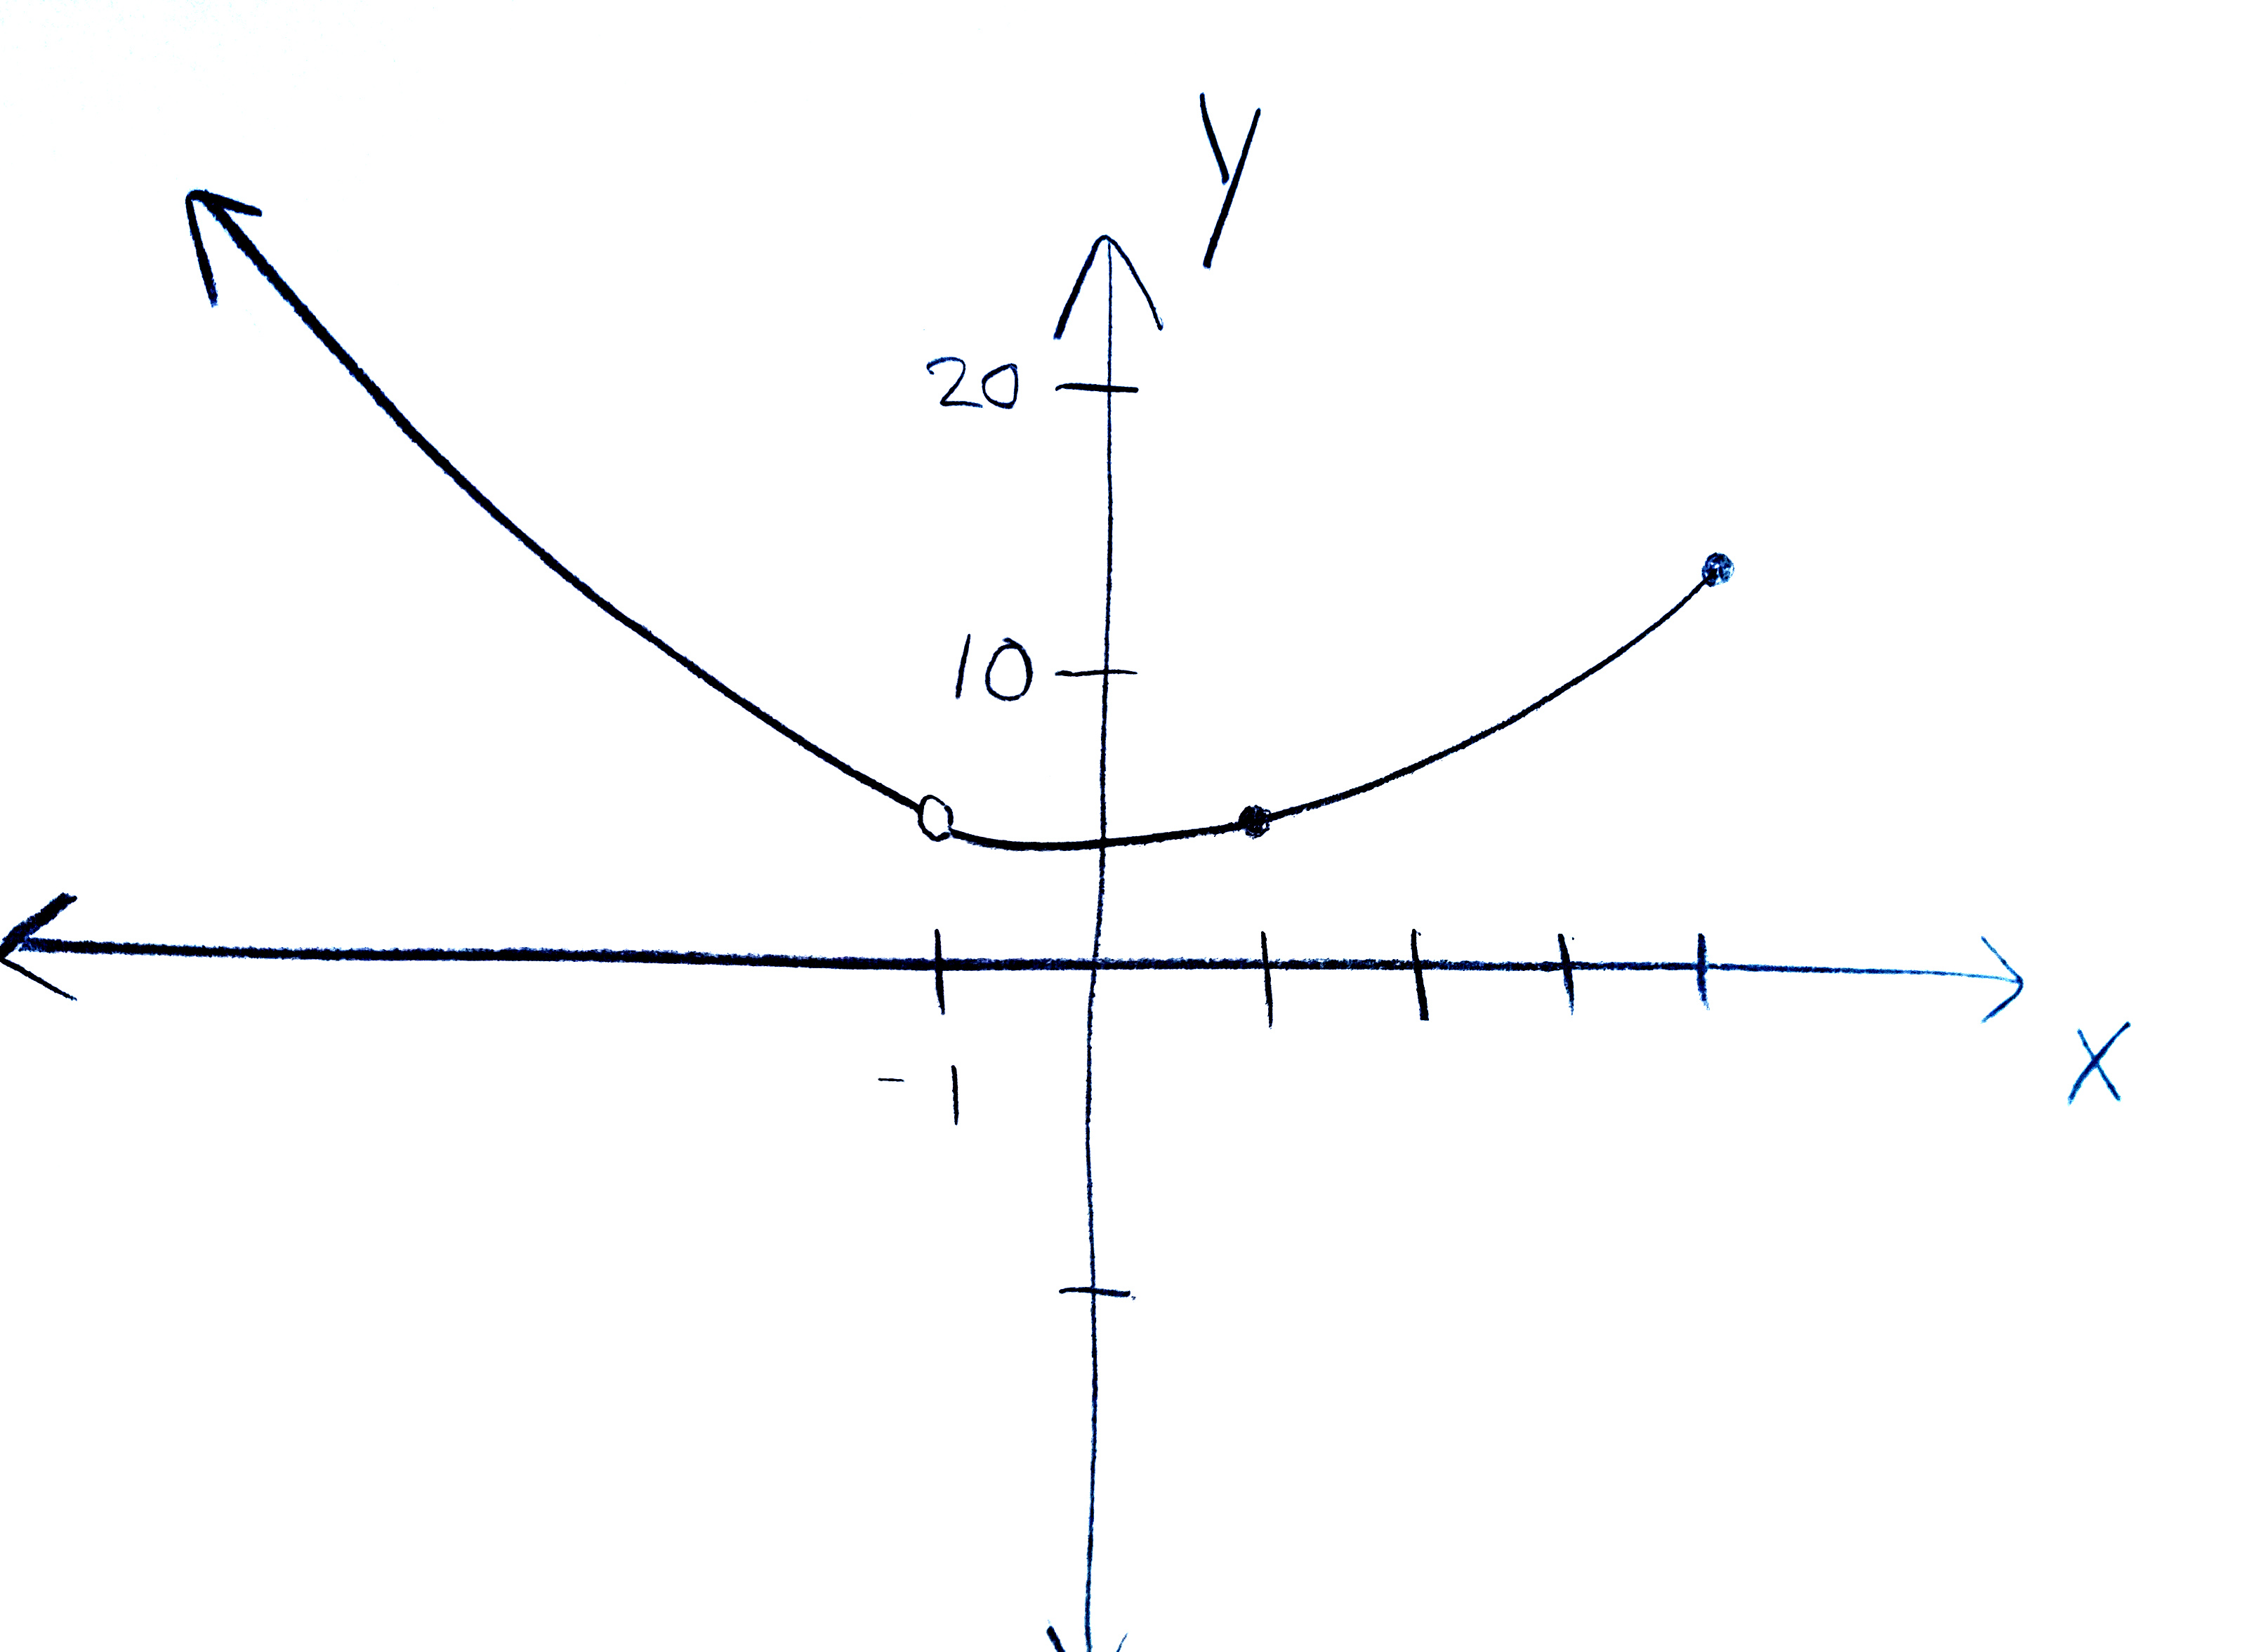
\includegraphics[scale=0.09]{images/cont-practice-inverted}
  \vspace{-2in}
\end{ex}
\begin{thrm}
  Properties of (facts about) continuous functions:
  \begin{enumerate}
    \item The constant function
    \item The identity function

    If $f$ and $g$ are continuous at $x=p$, then:
    \item $f(x)^n$
    \item $f \pm g$
    \item $fg$
    \item $f/g$
  \end{enumerate}
\end{thrm}
%%%%%%%%%%%%%%%%%%%%%%%%%%%%%%%%%%%%%%%%%%%%%%%%%%
\end{document}
